\subsection{Kiểm chứng mã giảm giá và điểm thưởng}
\begin{table}[htbp]\centering\small
\begin{minipage}[t]{.69\linewidth}\vspace{0pt}
\begin{tabularx}{\linewidth}{|p{.18\linewidth}|X|}\hline
\textbf{Ca} & \textbf{Nội dung kiểm tra}\\\hline
KM-01 & Chuẩn hóa hoa/thường, khoảng trắng; mã thiếu/hết hạn/inactive bị từ chối.\\\hline
KM-02 & 120.000đ giảm 10\% còn 108.000đ; làm tròn đúng và không giảm vượt tổng.\\\hline
KM-03 & Mã sai không tạo đơn hoặc trừ nguyên liệu.\\\hline
KM-04 & PAID ghi số dư và một EARN khớp amount sau giảm; dưới ngưỡng không ghi EARN.\\\hline
KM-05 & Request/IPN lặp không nhân đôi điểm; unique chặn EARN trùng.\\\hline
KM-06 & Lỗi cộng điểm rollback settlement; đổi món chỉ cộng điểm trên tiền mới.\\\hline
\end{tabularx}
\end{minipage}\hfill
\begin{minipage}[t]{.27\linewidth}\vspace{0pt}
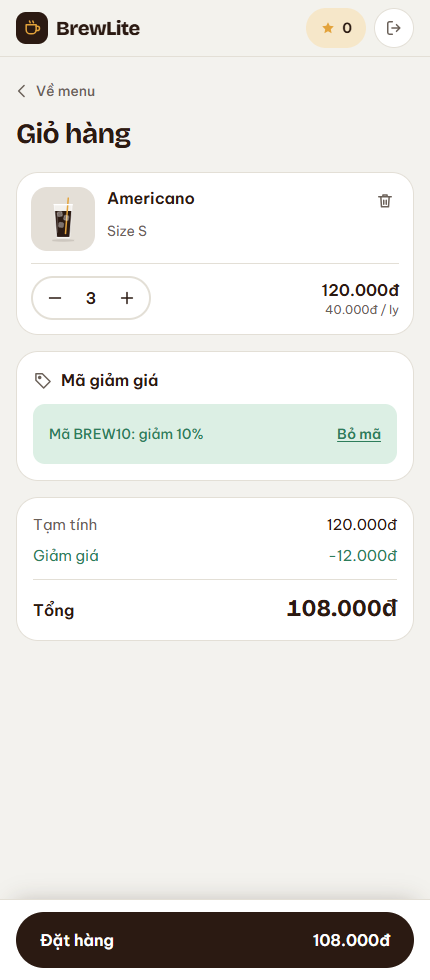
\includegraphics[width=\linewidth]{assets/promotions/voucher-ui-fixture.png}
\end{minipage}
\caption{Tiêu chí kiểm chứng khuyến mãi/điểm và giỏ hàng áp mã với API fixture}
\end{table}

Unit test nằm tại \path{src/promotions/discount.spec.ts}; API test nằm trong promotions, loyalty, staff-orders, VNPay và payment-exchange. Các bộ này kiểm đồng thời kết quả phản hồi, User.loyaltyPoints và dòng sổ EARN. Phạm vi kết quả đã xác minh dùng chung với mục~\ref{sec:inventory-tests}; phần này không bổ sung một số liệu chạy mới. Ảnh giỏ hàng chỉ kiểm chứng hiển thị giảm giá với dữ liệu thử.
